\documentclass[10 pt,usenames,dvipsnames, oneside]{article}
\usepackage{../../../modelo-ensino-medio}



\begin{document}

\begin{center}
  \begin{minipage}[l]{3cm}

\includegraphics[width=2cm]{logo}    
\end{minipage}\hfill
\begin{minipage}[r]{.8\textwidth}
 {\Large \scshape Atividade: Concentração de álcool no sangue}  
\end{minipage}
\end{center}
\vspace{.2cm}

\ifdefined\prof
%Habilidades da BNCC
% \begin{objetivos}
% \item 
% \end{objetivos}

%Caixa do Para o Professor
\begin{goals}
%Objetivos específicos
\begin{enumerate}
\item Contextualizar uma inequação do segundo grau.
\end{enumerate}

\tcblower

%Orientações e sugestões
\begin{itemize}
\item Professor, faça o aluno perceber que a desigualdade apresentada aqui não é mais do tipo $ax^2+bx+c>0$ c mas do tipo $ax^2+bx+c>d$.
\item Tranquilize seus alunos com relação aos valores dessa atividade. Eles podem achar que estão seguindo pelo caminho errado porque estão acostumados a valores inteiros, no entanto, lembre-os que os valores encontrados em situações reais são assim mesmo.  
\end{itemize}
\end{goals}

\bigskip
\begin{center}
{\large \scshape Atividade}
\end{center}
\fi
\textit{(Adaptada de Cespe - PRF)}

Considere que o nível de concentração de álcool na corrente sanguínea, em $g/L$, de uma pessoa, em função do tempo $t$, em horas, seja expresso por $N =-0{,}008(t^2 - 35t + 34)$. Considere, ainda, que essa pessoa tenha começado a ingerir bebida alcoólica a partir de $t = t_0$ ($N(t_0) = 0$), partindo de um estado de sobriedade, e que tenha parado de ingerir bebida alcoólica em $t = t_1$, voltando a ficar sóbria em $t = t_2$. Considere, por fim, a figura a seguir, que apresenta o gráfico da função $N(t)$ para $t \in [t_0, t_2]$. 


\begin{figure}[H]
\centering
\noindent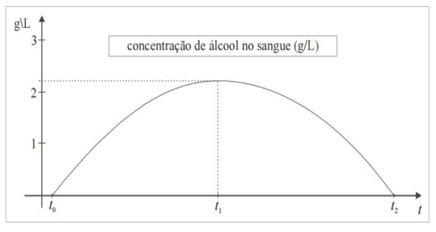
\includegraphics[width=260bp]{alcool}
\end{figure}

Com base nessas informações e tomando $24{,}3$ como valor aproximado de $\sqrt{589}$, analise a afirmativa a seguir:

“O nível de concentração de álcool na corrente sanguínea da pessoa em questão foi superior a $1 g/L$ por pelo menos $23$ horas.”

\ifdefined\prof
\begin{solucao}

Sim. A inequação base do problema é $-0{,}008(t^2-35t + 34)>1.$ A solução para ela é o intervalo $(5{,}35;29{,}65)$. Calculando a diferença temos $24{,}3$, portanto, superior a $23$ hrs

\end{solucao}
\fi

\end{document}